\documentclass{beamer}
\usepackage{progressbar, tcolorbox, CJKutf8, hyperref, multicol, pdfpages, graphicx, xcolor, blindtext, tikz, smartdiagram, listings, tikz}
\usepackage[absolute,overlay]{textpos}
\usepackage[backend=bibtex,style=numeric,sorting=none]{biblatex}
\usetikzlibrary{positioning, calc, shapes.multipart, shapes.arrows, fit, backgrounds}

\hypersetup{
    colorlinks=true,
    linkcolor=blue,
    filecolor=magenta,      
    urlcolor=blue,
    }

    \definecolor{mygreen}{rgb}{0,0.6,0}
    \definecolor{mygray}{rgb}{0.5,0.5,0.5}
    \definecolor{mymauve}{rgb}{0.58,0,0.82}
    \definecolor{mycolor}{rgb}{0.1, 0.78, 0.78}


    \lstset{ 
      backgroundcolor=\color{white},   % choose the background color; you must add \usepackage{color} or \usepackage{xcolor}; should come as last argument
      basicstyle=\ttfamily\footnotesize,% the size of the fonts that are used for the code
      breakatwhitespace=false,         % sets if automatic breaks should only happen at whitespace
      breaklines=true,                 % sets automatic line breaking
      captionpos=b,                    % sets the caption-position to bottom
      commentstyle=\color{mygreen},    % comment style
      deletekeywords={...},            % if you want to delete keywords from the given language
      escapeinside={\%*}{*)},          % if you want to add LaTeX within your code
      extendedchars=true,              % lets you use non-ASCII characters; for 8-bits encodings only, does not work with UTF-8
      frame=single,	                   % adds a frame around the code
      keepspaces=true,                 % keeps spaces in text, useful for keeping indentation of code (possibly needs columns=flexible)
      keywordstyle=\color{magenta},        % keyword style
      morekeywords={FROM, RUN, ENV, USER, WORKDIR, CMD, EXPOSE, ADD, COPY, sudo, curl, chmod, ln, git, cd},
                                       % if you want to add more keywords to the set
      numbers=left,                    % where to put the line-numbers; possible values are (none, left, right)
      numbersep=5pt,                   % how far the line-numbers are from the code
      numberstyle=\tiny\color{mygray}, % the style that is used for the line-numbers
      rulecolor=\color{black},         % if not set, the frame-color may be changed on line-breaks within not-black text (e.g. comments (green here))
      showspaces=false,                % show spaces everywhere adding particular underscores; it overrides 'showstringspaces'
      showstringspaces=false,          % underline spaces within strings only
      showtabs=false,                  % show tabs within strings adding particular underscores
      stepnumber=1,                    % the step between two line-numbers. If it's 1, each line will be numbered
      stringstyle=\color{mymauve},     % string literal style
      tabsize=4,	                     % sets default tabsize to ˋ spaces
      title=\lstname
    }

\graphicspath{ {./images/} }
\usetheme{AnnArbor}
\addbibresource{slide.bib}
\usetikzlibrary{positioning, calc, shapes.multipart, shapes.arrows, fit, backgrounds}

\definecolor{dockerColor}{RGB}{13, 183, 237}
\definecolor{secureColor}{RGB}{10, 191, 83}
\definecolor{aquamarine}{rgb}{0.5, 1.0, 0.83}
\definecolor{aquamarine2}{rgb}{0.2, 1.0, 0.53}
\definecolor{gold}{rgb}{1.0, 0.84, 0.0}

\title[Container Security]{The Container Security in Healthcare Data Exchange System}
\subtitle{Bachelor's degree graduation project}
\author[Chih-Hsuan Yang]{Chih-Hsuan Yang \\
{\small Advisor: Chun-I Fan} \\ 
{Team {\color{red} \textbf{18}}.}
}
\institute{NSYSU}
\date{}

\AtBeginSection[]{
  \begin{frame}
  \vfill
  \centering
  \begin{beamercolorbox}[sep=8pt,center,shadow=true,rounded=true]{title}
    \usebeamerfont{title}\insertsectionhead\par%
  \end{beamercolorbox}
  \vfill
  \end{frame}
}

\def\checkmark{\tikz\fill[scale=0.4](0,.35) -- (.25,0) -- (1,.7) -- (.25,.15) -- cycle;} 

\begin{document}
\begin{CJK*}{UTF8}{bsmi}

    \begin{frame}
        \titlepage
    \end{frame}

    \begin{frame}{Outline}
        \begin{multicols}{2}
            \tableofcontents
        \end{multicols}
    \end{frame}

    \section{Big picture}
    \begin{frame}
        \begin{columns}
            \begin{column}{0.30\textwidth}
                \centering
                \includegraphics[height=0.4\textheight, trim=150 100 100 100,clip]{container.jpg}
                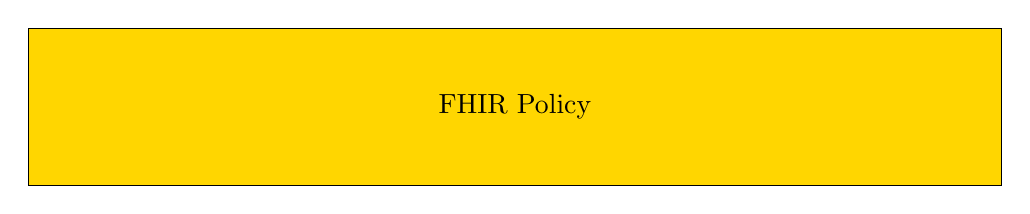
\begin{tikzpicture}
                    \tikzstyle{block} = [draw, rectangle, text width=\textwidth, text centered, minimum height=2cm, fill=gold]
                    \node [block, name = policy] {FHIR Policy};
                \end{tikzpicture}
                \includegraphics[width=\textwidth]{linux.png}
            \end{column}
            \begin{column}{0.30\textwidth}
                \centering
                \includegraphics[height=0.3\textheight]{sick.png}\\
                \includegraphics[width=\textwidth, height=0.3\textheight]{mask.png}\\
                \includegraphics[height=0.3\textheight]{house.png}
            \end{column}
            \begin{column}{0.30\textwidth}
                \centering
                \includegraphics[height=0.3\textheight]{man.png}\\
                \includegraphics[width=\textwidth, height=0.3\textheight]{mask.png}\\
                \includegraphics[height=0.3\textheight]{people.png}
            \end{column}
        \end{columns}
    \end{frame}

    \begin{frame}
        \begin{columns}
            \begin{column}{0.30\textwidth}
                \centering
                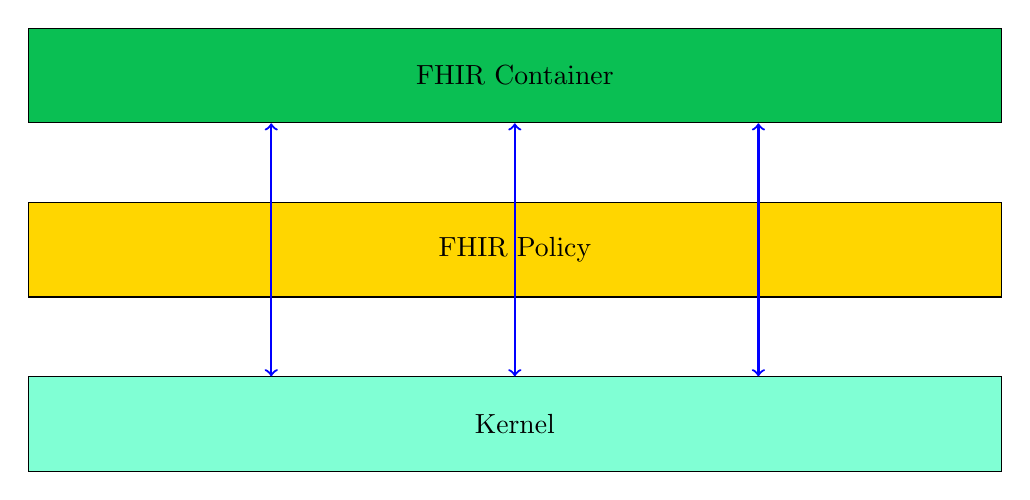
\begin{tikzpicture}
                    \tikzstyle{block} = [draw, rectangle, text width=\textwidth, text centered, minimum height=1.2cm, fill=gold]
                    \node [block, name = policy] {FHIR Policy};
                    \node [block, name = container, above= of policy, fill=secureColor] {FHIR Container};
                    \node [block, name = kernel, below= of policy, fill=aquamarine] {Kernel};
                    \draw [thick, <->, blue] ($(container.south west)!0.25!(container.south east)$) -- ($(kernel.north west)!0.25!(kernel.north east)$);
                    \draw [thick, <->, blue] ($(container.south west)!0.5!(container.south east)$) -- ($(kernel.north west)!0.5!(kernel.north east)$);
                    \draw [thick, <->, blue] ($(container.south west)!0.75!(container.south east)$) -- ($(kernel.north west)!0.75!(kernel.north east)$);
                \end{tikzpicture}
                \newline
                Normal
            \end{column}
            \begin{column}{0.30\textwidth}
                \centering
                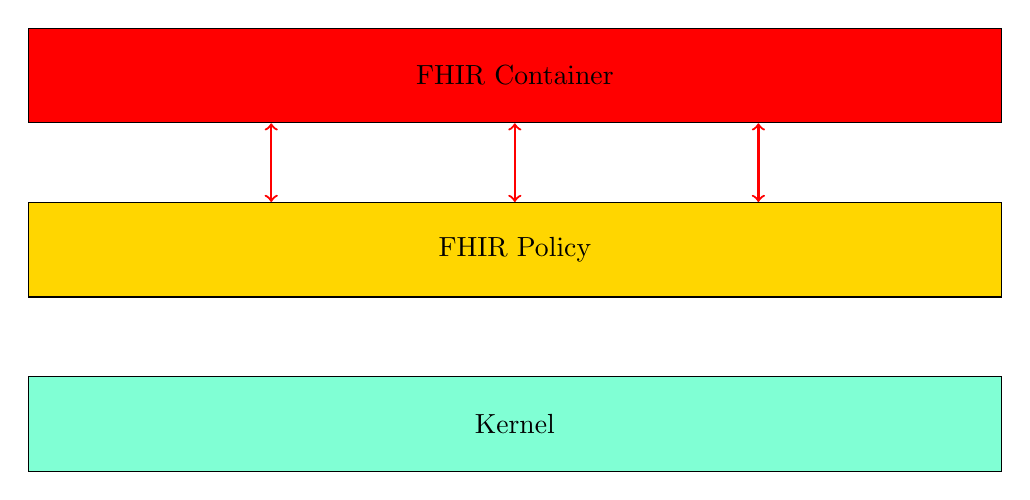
\begin{tikzpicture}
                    \tikzstyle{block} = [draw, rectangle, text width=\textwidth, text centered, minimum height=1.2cm, fill=gold]
                    \node [block, name = policy] {FHIR Policy};
                    \node [block, name = container, above= of policy, fill=red] {FHIR Container};
                    \node [block, name = kernel, below= of policy, fill=aquamarine] {Kernel};
                    \draw [thick, <->, red] ($(container.south west)!0.25!(container.south east)$) -- ($(policy.north west)!0.25!(policy.north east)$);
                    \draw [thick, <->, red] ($(container.south west)!0.5!(container.south east)$) -- ($(policy.north west)!0.5!(policy.north east)$);
                    \draw [thick, <->, red] ($(container.south west)!0.75!(container.south east)$) -- ($(policy.north west)!0.75!(policy.north east)$);
                \end{tikzpicture}
                \newline
                Load time check failed
            \end{column}
            \begin{column}{0.30\textwidth}
                \centering
                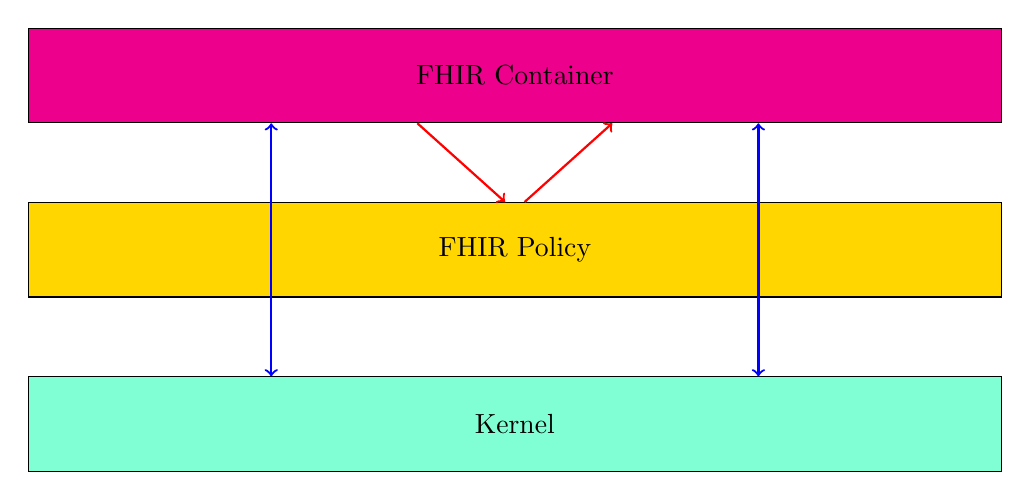
\begin{tikzpicture}
                    \tikzstyle{block} = [draw, rectangle, text width=\textwidth, text centered, minimum height=1.2cm, fill=gold]
                    \node [block, name = policy] {FHIR Policy};
                    \node [block, name = container, above= of policy, fill=magenta] {FHIR Container};
                    \node [block, name = kernel, below= of policy, fill=aquamarine] {Kernel};
                    \draw [thick, <->, blue] ($(container.south west)!0.25!(container.south east)$) -- ($(kernel.north west)!0.25!(kernel.north east)$);
                    \draw [thick, ->, red] ($(container.south west)!0.40!(container.south east)$) -- ($(policy.north west)!0.49!(policy.north east)$);
                    \draw [thick, <-, red] ($(container.south west)!0.60!(container.south east)$) -- ($(policy.north west)!0.51!(policy.north east)$);
                    \draw [thick, <->, blue] ($(container.south west)!0.75!(container.south east)$) -- ($(kernel.north west)!0.75!(kernel.north east)$);
                \end{tikzpicture}
                \newline
                Run time injected
            \end{column}
        \end{columns}
    \end{frame}

    \section{Demo}
    \begin{frame}{Architecture: on the same machine
        }\centering
        \begin{tikzpicture}
            \tikzstyle{block} = [draw, rectangle, text width=.8\textwidth, text centered, minimum height=1.2cm, fill=gold]
            \node [block, name = fhir_policy, above left=3cm and 0cm, fill=gold, text width=.36\textwidth] at (kernel) {FHIR Policy};
            \node [block, name = vic_policy, above right=3cm and 0cm, fill=secureColor, text width=.36\textwidth] at (kernel) {Victim Policy};
            \node [block, name = container, above= 2.5cm of fhir_policy, fill=magenta, text width=.36\textwidth] at (fhir_policy) {FHIR Container\\ {\footnotesize(isolated process)}};
            \node [block, name = victim, above= 2.5cm of vic_policy, fill=secureColor, text width=.36\textwidth] at (vic_policy) {Victim\\ {\footnotesize(isolated process)}};
            \node [block, name = docker, fill=dockerColor, above=4.5cm] at (kernel) {Docker Engine};
            \node [block, name = kernel, fill=aquamarine] {Kernel};
        \end{tikzpicture}
    \end{frame}

    \begin{frame}
        \centering
        \Huge Live demo.
    \end{frame}

    \section{Why this}
    \begin{frame}{Why this idea has not been proposed?}
        \begin{enumerate}
            \item Docker provides a general mask to containers, however, it does {\color{blue} \textbf{not have enough efficacy}} to protect the special container.
            \item Google used a sandbox to encapsulate, however, our researching target (IBM/FHIR) did {\color{red} \textbf{not support}} gVisor.
            \item This is a new issue in security, moreover, it must have much Linux kernel knowledge to interact with.
        \end{enumerate}
    \end{frame}

    \begin{frame}{Pros and Cons}
        \begin{table}[]
            \begin{tabular}{|l|l|l|}
                \hline
                            & Our proposal                          & Sandbox       \\ \hline
                General     & {\color{red} \textbf{solid}}      & flexible      \\ \hline
                Performance & {\color{mygreen} \textbf{efficiency}} & expensiveness \\ \hline
            \end{tabular}
        \end{table}
    \end{frame}

    \section{Statistic \& Performance}
    \begin{frame}
        \centering
        \includegraphics[width=\textwidth, height=\textheight]{hist.png}
    \end{frame}
    \begin{frame}
        \centering
        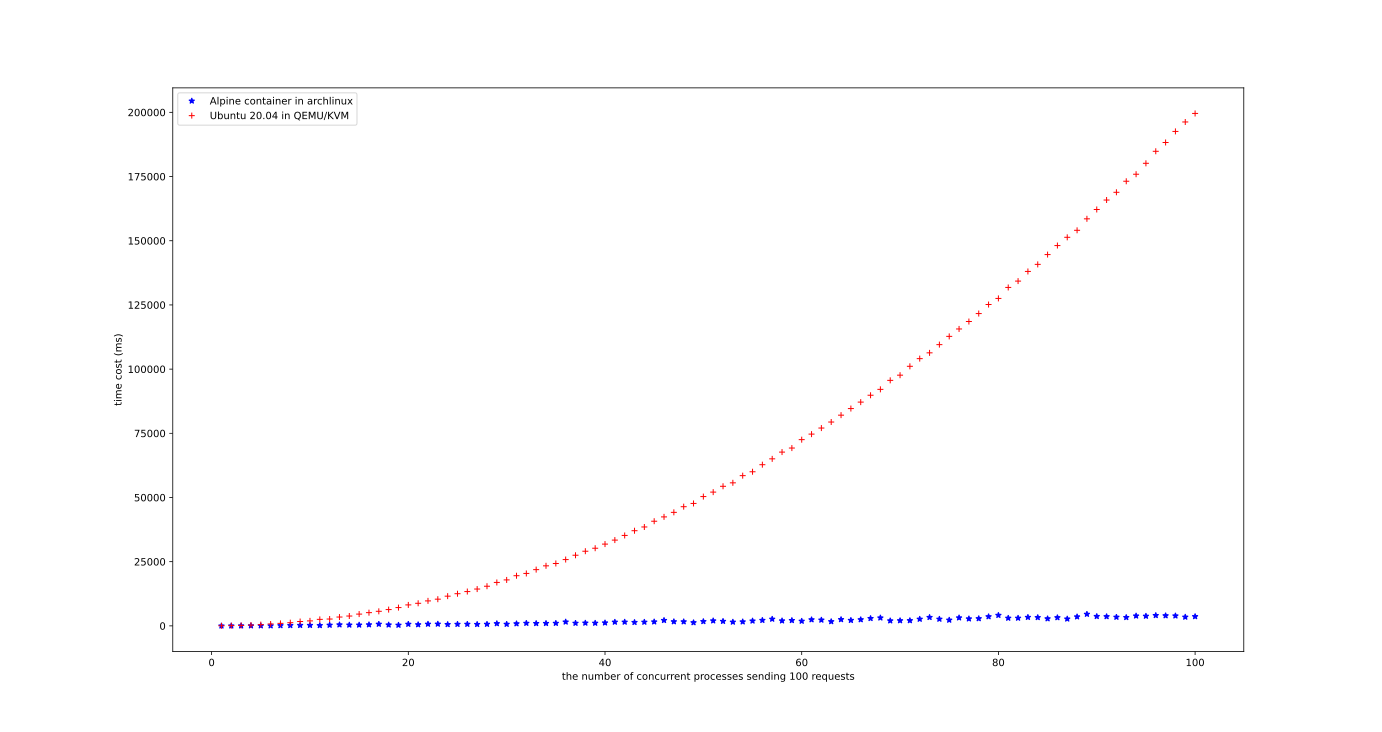
\includegraphics[width=\textwidth, height=\textheight]{concurrent.png}
    \end{frame}

    \begin{frame}{Conclusion}
        \begin{itemize}
            \item We propose a {\color{secureColor} \textbf{secure workflow}} for FHIR system.
            \item We benchmark the {\color{secureColor} \textbf{concurrent performance}} of container and virtual machine in FHIR system server.
            \item We provide a {\color{secureColor} \textbf{reliable statistic}} in FHIR system for Taiwan.
        \end{itemize}
    \end{frame}

\end{CJK*}
\end{document}